\documentclass[]{article}

\usepackage{amssymb}
\usepackage{amsmath}
\usepackage{graphicx}
\usepackage{amsthm}
\newtheorem{theorem}{Theorem}
\newcommand{\state}{\ensuremath{\mathbf{x}}}
\newcommand{\control}{\ensuremath{\mathbf{u}}}
\newcommand{\costate}{\mathbf{p}}
\newcommand{\multiplier}{\mathbf{\lambda}}
%\newcommand{\costate}{\mathbf{\lambda}}
%\newcommand{\multiplier}{\mathbf{\nu}}
\newcommand{\E}[1]{\mathbb{E}[#1]}
\newcommand{\V}[1]{\mathbb{V}[#1]}
\newcommand{\mean}{\mathbf{m}}
\newcommand{\cov}{P}
\newcommand{\std}{S}
\newcommand{\sample}{\ensuremath{\mathbf{z}}}
% Title Page
\title{Optimal Control of an Entry Vehicle for Minimum Propellant Powered Descent Ignition on Mars}



\begin{document}
\author{Connor D. Noyes\thanks{Ph.D. Candidate, Department of Mechanical and Aerospace Engineering, University of California, Irvine, 92697} \ and Kenneth D. Mease\thanks{Professor Emeritus, Department of Mechanical and Aerospace Engineering, University of California, Irvine, 92697}}
\maketitle

\section{Optimal Control Theory}

The field of Hybrid Optimal Control Theory is concerned with optimal control problems including multiple phases, in which the number of states and controls, as well as the dynamics and other constraints, may vary, and in which the number and order of the phases are optimization variables. Our problem is a special case in which the number and ordering of the phases are fixed. Additionally, the phase transition is called autonomous because they are uniquely determined by the state just prior to the transition. 

Notation: gradients are row vectors, the Jacobian of a function mapping $m$ inputs to $n$ outputs is an $n\times m$ matrix.

In each phase, there is a costate vector $\costate_i$ associated with each state vector $\state_i$. We consider an objective of the form $J = \Phi(t_f, \mathbf{x}(t_f))$. Because there is no Lagrange term, the Hamiltonian in the $i^{\mathrm{th}}$  phase is $H_i = \costate_i^T\dot{\mathbf{x}}_i$.

The final state is constrained to the manifold $C\state_2(t_f) = \mathbf{0}$ where C is a $p\times n$ matrix designed to pick off the desired states. At the phase transition, the state may undergo a nonlinear transformation $T: \mathbb{R}^{n_1} \to \mathbb{R}^{n_2}$. Let $\Psi(\state_1,\state_2) = T(\state_1(t_s))-\state_2(t_s)$.

The final time and duration of each phase is free. Let $t_s$ be the time of the phase transition. Adjoining the terminal constraint and the state transformation to the objective via Lagrange multipliers $\multiplier, \nu$ yields the endpoint function 
\begin{equation}
G = \Phi + \multiplier^TC\state_2(t_f) + \nu^T\Psi.
\end{equation} 
The augmented objective function is 
\begin{align}
J' = G(\state_1(t_s), \state_2(t_s), \state_2(t_f)) + \int_{t_0}^{t_s}\left[H(t,\state_1,\control_1,\costate_1) - \costate_1^T\dot{\state}_1\right]\mathrm{d}t \\
+ \int_{t_s}^{t_f}\left[H(t,\state_2,\control_2,\costate_2) - \costate_2^T\dot{\state}_2\right]\mathrm{d}t \nonumber
\end{align}
and its first differential is
\begin{align}
dJ' = very\,\,long\,\,tbd...
%( G_{t_f} + G_x\dot{\state}_f)dt_f + (G_x-\costate_f^T)\delta x_f \\+ \int_{t_0}^{t_f}\left[(H_x+\dot{\costate}^T)\delta\state + H_u\delta \control\right]\mathrm{d}t
\end{align}
from which we find the following necessary conditions
\begin{align}
\dot{\state} &= H_p \\
-\dot{\costate}^T &= H_x \\
\costate_1^T(t_s) &= -\nu^T\Psi_{x_1} = -\nu^TT_{x_1}\\
\costate_2^T(t_s) &= \nu^T\Psi_{x_2} = -\nu^T\\
\costate_2^T(t_f) &= G_x =\Phi_x + \multiplier^TC\\
H_1(t_s) &= H_2(t_s) \\
H_2(t_f) &= 0 \\
H(\state^*,\control^*,\costate^*, t) &\le H(\state^*,\control,\costate^*, t) \\
C\state(t_f) &= \mathbf{0} \\
\Psi(x_1(t_s),x_2(t_s)) &= 0.
\end{align}
 We can combine the two costate boundary conditions at $t_s$ to determine a direct relationship between the costates before and after the transition, which is $\costate_1(t_s) = T_{x_1}^T\costate_2(t_s)$.
The simplified necessary conditions are 
%\begin{align}
%\dot{\state} &= f(x,u) \\
%\state_1(t_0) & = x_0\\
%\state_2(t_s) &= T(\state_1(t_s)) \\
%C\state_2(t_f) &= \mathbf{0} \\
%-\dot{\costate} &= f^T_x(x,u)\costate \\
%\costate_1(t_s) &= T^T_{x_1}\costate_2(t_s) \label{eq_costate_transition} \\
%\costate_2(t_s) &= -\nu\\
%\costate_2(t_f) &=\Phi^T_x + C^T\multiplier\\
%H_1(t_s) &= H_2(t_s) \\
%H_2(t_f) &= 0 \\
%H_u &= \mathbf{0},
%\end{align}
\begin{align}
&\dot{\state} = f(x,u) \\
&\state_1(t_0)  = x_0\\
&\state_2(t_s) = T(\state_1(t_s)) \\
C&\state_2(t_f) = \mathbf{0} \\
-&\dot{\costate} = f^T_x(x,u)\costate \\
&\costate_1(t_s) = T^T_{x_1}\costate_2(t_s) \label{eq_costate_transition} \\
&\costate_2(t_s) = -\nu\\
&\costate_2(t_f) =\Phi^T_x + C^T\multiplier\\
&H_1(t_s) = H_2(t_s) \\
&H_2(t_f) = 0 \\
&H(\state^*,\control^*,\costate^*, t) \le H(\state^*,\control,\costate^*, t)
%&H_u = \mathbf{0},
\end{align}
%a system of $ n_1 + 2n_2 + p + 2 $ variables in $\state,\,\costate,\,\multiplier,\nu,\,t_s,\,\mathrm{and}\,t_f$.


\section{Solutions to Two Phase Optimal Control Problem}

Numerical solutions to propellant-optimal entry + powered descent problem are used to inform aspects of our guidance approach. The problem is posed under different conditions to examine how the solutions change. In all scenarios, the optimal control objective is minimizing the propellant to land the vehicle. A range of entry flight path angles was considered.


%The control variable during the entry phase is taken to be the bank angle rate and the bank angle is added as a state variable. This allows me to recover different parametrizations of interest - setting the rate high allows for bang-bang solutions, while setting the max rate to zero recovers constant bank angle solutions. And naturally when the rate is set to something the vehicle can track, the trajectories show more reasonable responses.

\subsection{Propellant Optimal Deceleration}
In this formulation, there is no constraint on the horizontal position at the termination of the entry phase, nor at the termination of the SRP phase. In theory this should eliminate any bank reversals, since the vehicle heading at ignition does not play any role in the propellant cost. The solution to this problem provides a lower bound on the propellant required with position constraints included. Numerically, if the bank angle reversals may occur instantaneously, 

Consider the minimal state vector comprising only altitude, velocity, and flight path angle during entry $x = [r, v, \gamma]$. During powered descent the state vector must also include the vehicle mass, and the states are written in cartesian coordinates.

During entry $\state = [r, v, \gamma]$, while during powered descent $\state = [z, \dot{z}, \dot{d}, m]=[r-r_{target}, v\sin\gamma, v\cos\gamma, m]$. The Hamiltonian in each phase is
\begin{align}
H_1 &= p_hv\sin\gamma - p_v(D+g\sin\gamma) + p_{\gamma}\left(\frac{L}{v}u + (\frac{v}{r}-\frac{g}{v})\cos\gamma\right) \\
H_2 &= p_z\dot{z} - p_{\dot{z}}(\frac{T_z}{m}-g) + p_{\dot{d}}\frac{T_d}{m} - p_mkT
\end{align}

The control appears linearly in $H_1$, and thus, the optimal bank angle profile is bang-bang in nature with switching function $p_{\gamma}$. (This is because $\frac{\partial H_1}{\partial u} = p_{\gamma}\frac{L}{v}$ and $L/v > 0$).
\begin{figure}[h!]
	\centering
	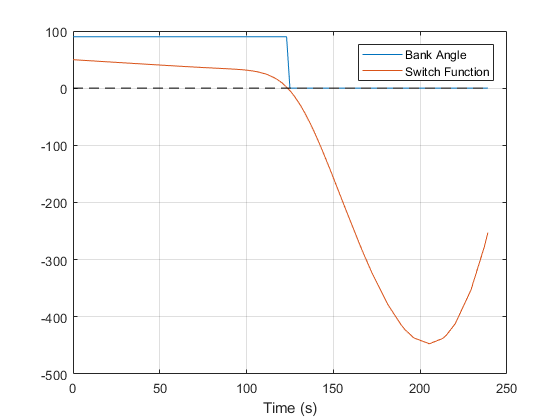
\includegraphics[width=1\textwidth]{switch_function}
	\caption{The costate associated with the state variable $\gamma$  determines the bank angle switching sequence during entry.}
%	\label{fig_pmf_vs_alt}
\end{figure}
The costate dynamics during the entry phase are 
\begin{align}
-\dot{p}_r &= p_v\frac{D}{h_s} - p_{\gamma}\left(\frac{L}{vh_s}u + (\frac{v}{r^2}-\frac{2g}{vr})\cos\gamma\right) \\
 -\dot{p}_v &= p_rv\sin\gamma - p_v\frac{2D}{v} + p_{\gamma}\left(\frac{L}{v^2}u + (\frac{1}{r}-\frac{g}{v^2})\cos\gamma\right) \\
 -\dot{p}_{\gamma}&= p_rv\cos\gamma - p_vg\cos\gamma-p_{\gamma}\left((\frac{v}{r}-\frac{g}{v})\sin\gamma\right).
\end{align}
Due to the nonlinearity and coupling of the costate trajectories, it is difficult to determine analytically how many times the optimal bank angle profile will switch between its bounds. We proceed with numerical solutions to learn more about their structure.

The solutions to this problem are characterized by bang-bang bank profiles with a single switch from lift down to lift up. The steeper the entry flight path angle, the earlier the switch to lift up.  
Dependence of the optimal propellant as well as ignition states on EFPA is fairly weak. The thrust profile during SRP is always at its maximum value. 

\begin{figure}[h!]
	\centering
	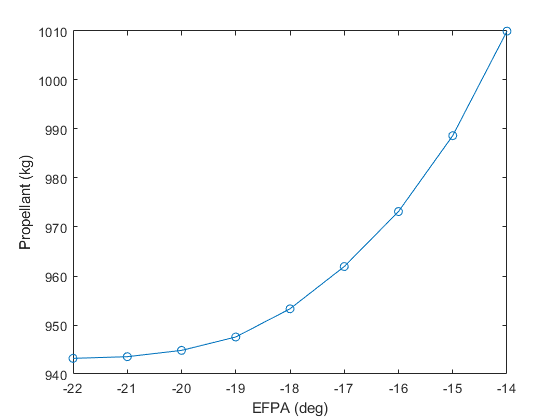
\includegraphics[width=0.8\textwidth]{prop_vs_efpa}
	\caption{The EFPA has a weak impact on the optimal propellant.}
%	\label{fig_pmf_vs_alt}
\end{figure}
\begin{figure}[h!]
	\centering
	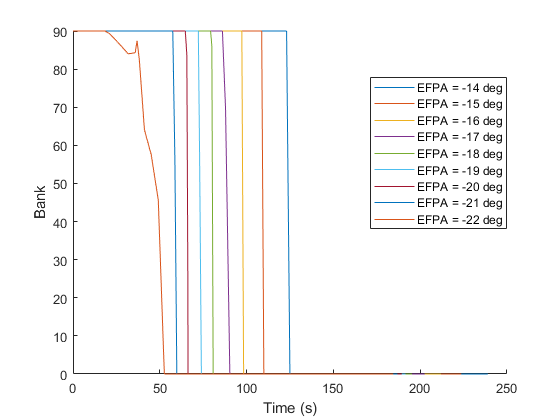
\includegraphics[width=0.8\textwidth]{bank_profiles_vs_efpa}
	\caption{The propellant-optimal bang-bang bank profiles for different entry flight path angles.}
%	\label{fig_pmf_vs_alt}
\end{figure}
\begin{figure}[h!]
	\centering
	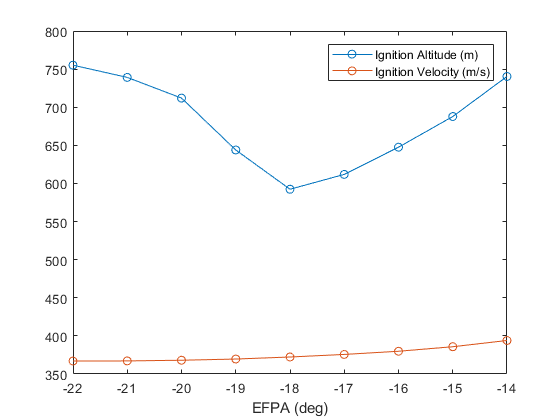
\includegraphics[width=0.8\textwidth]{ignition_vs_efpa}
	\caption{Optimal ignition occurs at very low altitudes, less than 1 km above the target altitude. The EFPA has a very weak impact on the ignition conditions when no horizontal target is imposed.}
%	\label{fig_pmf_vs_alt}
\end{figure}

\subsubsection{Minimum Altitude Constrained Solutions}

Because our past work has shown that the minimum ignition altitude plays an important role in determining the optimal ignition state, I sweep the value of this constraint from 0 (unconstrained) to +5 (or+10) km above the target altitude. I considered a fixed, nominal EFPA of -15.75 degrees. 

The bank angle profiles remain single switch. One change in the structure of the solution in the presence of an active minimum altitude constraint, is that the costate relationship given by Eq.~\ref{eq_costate_transition} no longer holds. 
Another difference is the thrust profile during powered descent is no longer maximal for the entire SRP phase. Instead, many solutions have an initial minimum thrust arc.  
%\subsubsection{No Bank Angle Parametrization}
%Bank angle rate limit is 10 deg/s.
%
%No Control Parametrization, Fixed EFPA
%Solutions are bang-bang with an initial lift-down arc, followed by a switch to lift up.
%
%No Control Parametrization, Optimized EFPA
%
%\begin{figure}[h!]
%	\centering
%	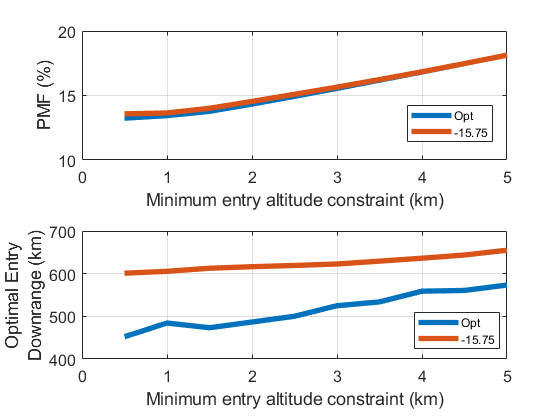
\includegraphics[width=1\textwidth]{pmf_vs_alt} 
%	\caption{The minimum altitude has a strong impact on both the PMF and optimal entry downrange distance.}
%	\label{fig_pmf_vs_alt}
%\end{figure}
%\begin{figure}[h!]
%	\centering
%	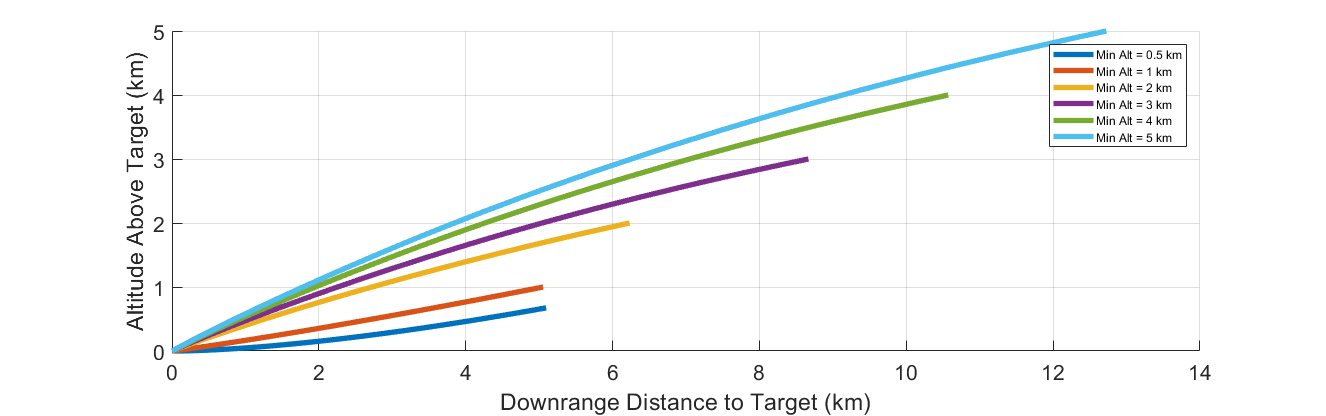
\includegraphics[width=1\textwidth]{srp} 
%	\caption{Geometry of propellant optimal trajectories for different values of the minimum ignition altitude. A 5 km constraint essentially doubles the optimal SRP downrange flown relative to the unconstrained trajectory. }
%	\label{fig_srp}
%\end{figure}
%
%\subsubsection{Constant Bank Angle Parametrization}
%Optimized EFPA solutions are constant full lift up (zero bank). Across all altitudes, the optimal EFPA was steeper than our nominal -15.75, and hence the optimized EFPA curve is always superior to the fixed EFPA curve. 
%\begin{figure}[h!]
%	\centering
%	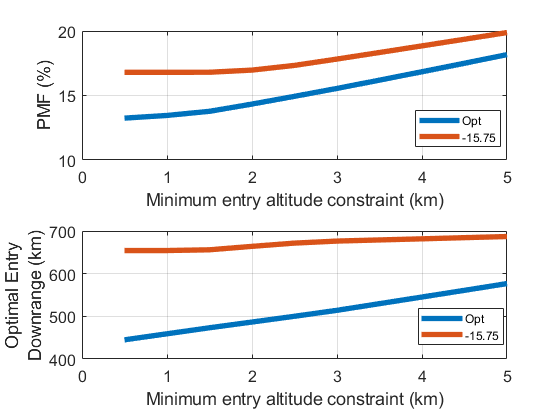
\includegraphics[width=1\textwidth]{pmf_vs_alt_constant_bank} 
%	\caption{The minimum altitude has a strong impact on both the PMF and optimal entry downrange distance. These plots are for the constant bank angle parametrization. }
%	\label{fig_pmf_constant_bank}
%\end{figure}
%\begin{figure}[h!]
%	\centering
%	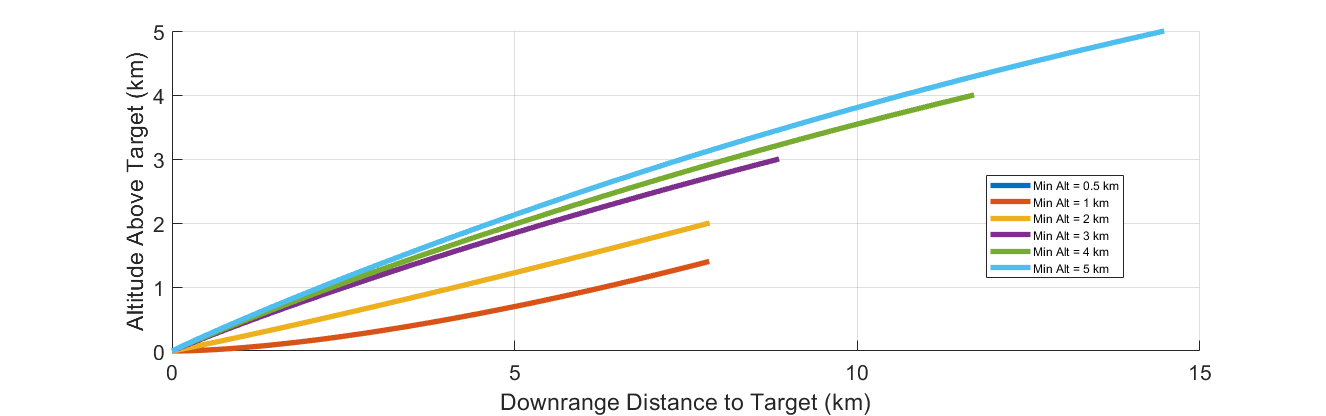
\includegraphics[width=1\textwidth]{srp_constant_bank} 
%	\caption{Geometry of propellant optimal trajectories for a constant bank angle parametrization and different values of the minimum ignition altitude. A 5 km constraint essentially doubles the optimal SRP downrange flown relative to the unconstrained trajectory. }
%	\label{fig_srp_constant_bank}
%\end{figure}


\bibliography{bib}

\end{document}